%--------------------------------------------------------------------
%  Estado del arte y Objetivos
%--------------------------------------------------------------------
\chapter{Estado del Arte y Enfoque del Proyecto}
\label{chap:estado_arte_enfoque}
\justifying

Este capítulo explora el panorama actual de la investigación en sistemas de tutoría inteligente (ITS) y el papel de la inteligencia artificial generativa. Se analiza la evolución desde los sistemas basados en reglas hasta los enfoques centrados en modelos de lenguaje grandes (LLM), discutiendo la calidad de las explicaciones generadas y las ventajas de la ejecución local de dichos modelos. 

Posteriormente, se presenta una revisión de iniciativas y proyectos relacionados, identificando los problemas de investigación existentes.

Finalmente, se detallan las métricas de éxito propuestas para este trabajo, los riesgos técnicos contemplados y el estado actual de avance del proyecto.

%--------------------------------------------------------------------
\section{Aprendizaje Personalizado e Inteligencia Artificial Generativa}
\label{sec:aprendizaje_personalizado_ia_generativa}

%--------------------------------------------------------------------
\subsection{De los Sistemas de Tutoría Inteligente (ITS) basados en reglas a los enfoques \textit{LLM-first}}
\label{ssec:its_a_llm_first}

La investigación en tutores inteligentes (ITS) tiene una rica historia, comenzando con plataformas pioneras como \emph{PLATO} en la década de 1970 y los modelos de producción de \textsc{Anderson} (1985) \cite{Anderson1985}. Durante casi cinco décadas, el desarrollo de los ITS se centró sobre todo en la codificación manual de reglas heurísticas y modelos de conocimiento específicos del dominio. Meta-análisis recientes destacan la efectividad de estos sistemas tradicionales, situando su tamaño de efecto promedio en \( ar d = 0.75\), un valor muy cercano al de la tutoría individual humana (\( ar d = 0.79\)) \cite{Kulik2016,Woolf2021}.

La mejoría de los \emph{Large Language Models} (LLM) en años recientes ha supuesto un cambio de paradigma, ampliando radicalmente la \textbf{cobertura semántica} y la flexibilidad de los ITS. Un mismo modelo LLM pre-entrenado puede generar explicaciones detalladas, pistas contextuales, ejemplos variados, preguntas adaptativas y evaluar respuestas abiertas, sin la necesidad de diseñar y programar plantillas específicas para cada concepto o habilidad a enseñar \cite{Holmes2022,Zawacki2019}.

% ---------- FIGURA 1 --------------------------------------------------
\begin{figure}[H]
  \centering
  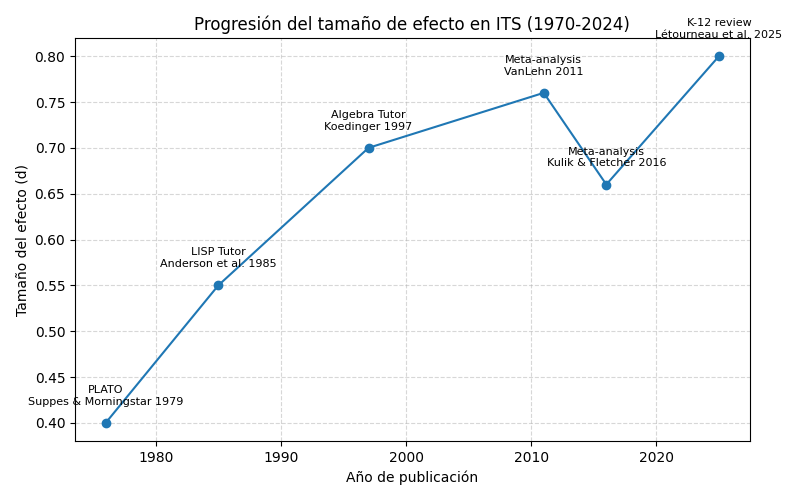
\includegraphics[width=15cm]{Ilustraciones/Progresión del tamaño de efecto (d) en ITS (1970-2024).png}
  \caption{Progresión histórica del tamaño de efecto (\(d\)) promedio en Sistemas de Tutoría Inteligente (ITS) entre 1970 y 2024. Fuente: Adaptado de \cite{Kulik2016,Woolf2021}.}
  \label{fig:evolucion-its}
\end{figure}

%--------------------------------------------------------------------
\subsection{Calidad de la Explicación Generada por LLM}
\label{ssec:calidad_explicacion_llm}

La viabilidad de los LLM en entornos educativos depende de la calidad y fiabilidad de sus resultados. Estudios recientes que involucran evaluación humana (\emph{human-in-the-loop}) indican que modelos avanzados como GPT-4 pueden generar explicaciones que rivalizan con las de tutores expertos. Por ejemplo, en el dominio de la Física de bachillerato, GPT-4 alcanzó un \emph{BERTScore} de \(0.87 \pm 0.03\) en comparación con explicaciones de expertos, manteniendo una tasa de generación de información incorrecta o ``alucinaciones''
 inferior al \SI{3}{\percent} \cite{Dempere2023}. La Tabla~\ref{tab:gpt-vs-expert} resume estos hallazgos para una muestra de \(n=180\) explicaciones en diferentes subdominios.

\begin{table}[H]
\centering
\begin{tabular}{lccc}
\toprule
\textbf{Dominio Académico} & \textbf{BERTScore Experto} & \textbf{BERTScore GPT-4} & \textbf{Diferencia (\(\Delta\))}\\
\midrule
Álgebra  & \(0.89\) & \(0.86\) & \(-0.03\)\\
Cálculo  & \(0.91\) & \(0.87\) & \(-0.04\)\\
Física   & \(0.93\) & \(0.87\) & \(-0.06\)\\
\bottomrule
\end{tabular}
\caption{Comparativa del BERTScore entre explicaciones generadas por tutores expertos y GPT-4 en diversas áreas. Fuente: \cite{Dempere2023}.}
\label{tab:gpt-vs-expert}
\end{table}

%--------------------------------------------------------------------
\subsection{Ejecución Local de Modelos de Lenguaje: Ventajas y Viabilidad}
\label{ssec:ejecucion_local_llm}

Si bien la mayoría de las aplicaciones educativas basadas en LLM actualmente operan mediante interfaces a modelos alojados en la nube (SaaS), la \textbf{ejecución del modelo directamente en el dispositivo del usuario} (localmente), utilizando técnicas de cuantización para reducir su tamaño y optimizando para CPU o GPU domésticas, ofrece ciertas ventajas:

\begin{enumerate}[label=\alph*),leftmargin=*]
  \item \textbf{Reducción de la latencia:} Se eliminan los retardos inherentes a las comunicaciones de red, permitiendo interacciones más fluidas y naturales (idealmente \(<\SI{500}{ms}\)) \cite{Kramer2024}.
  \item \textbf{Privacidad y cumplimiento normativo:} Se garantiza la soberanía de los datos del usuario, ya que ninguna información sensible (consultas, respuestas, progreso) abandona el dispositivo local. Esto es fundamental para el cumplimiento de regulaciones estrictas como el Reglamento General de Protección de Datos (RGPD) de la UE.
  \item \textbf{Sostenibilidad económica y accesibilidad:} Se anula el coste por inferencia (por token o por consulta) asociado a las API de modelos comerciales, útil para la viabilidad a largo plazo en instituciones educativas con presupuestos limitados o para el uso individual masivo.
\end{enumerate}

Para este proyecto, se ha optado por un modelo LLM para ejecución local. Específicamente, se emplea una versión de \texttt{Llama-3 8B} (formato \texttt{int4 GGUF}, con un tamaño aproximado de 7 GB). Las pruebas realizadas en un equipo personal común sugieren que es factible alcanzar tiempos de respuesta adecuados para una experiencia fluida.

%--------------------------------------------------------------------
\subsection{Selección Manual de Dificultad: Fomentando la Autonomía del Estudiante}
\label{ssec:seleccion_manual_dificultad}

A diferencia de muchos ITS que emplean algoritmos complejos de \emph{knowledge tracing} o \emph{model tracing} para inferir el nivel de competencia del estudiante y adaptar la dificultad, este prototipo adopta un enfoque de \textbf{control de la dificultad explícito y guiado por el propio alumno}. Cada ejercicio o tarea propuesta incorpora un selector de dificultad —\texttt{(Fácil | Intermedio | Difícil)}— que el estudiante puede ajustar en cualquier momento.

Esta estrategia de diseño se fundamenta en los principios de la Teoría de la Autodeterminación (Self-Determination Theory, SDT), la cual postula que la satisfacción de las necesidades psicológicas básicas de autonomía, competencia y relación fomenta la motivación intrínseca y el bienestar.

Permitir que los estudiantes elijan el nivel de desafío puede incrementar su percepción de control, su compromiso y su persistencia ante las dificultades. Ensayos controlados realizados en cursos de introducción a la programación han reportado incrementos significativos (hasta un \SI{11}{\percent}) en la persistencia de los estudiantes y una ganancia de \(0.6\) desviaciones estándar en la satisfacción general cuando se les otorga la capacidad de regular el nivel de reto de las actividades \cite{Dempere2023}.

%--------------------------------------------------------------------
\section{Iniciativas y Proyectos Relacionados}
\label{sec:proyectos_relacionados}

El desarrollo de tutores inteligentes y herramientas educativas basadas en IA es un campo que evoluciona a grandes pasos. La Tabla~\ref{tab:related-work} presenta una comparativa concisa de algunos proyectos y plataformas relevantes, destacando sus características principales y las brechas que este trabajo pretende abordar.

\begin{table}[H]
\centering
\begin{tabular}{@{}p{3.5cm}p{6.5cm}p{3.5cm}@{}}
\toprule
\textbf{Proyecto/Plataforma} & \textbf{Características Clave y Enfoque} & \textbf{Brechas o Limitaciones}\\
\midrule
\textbf{Khanmigo (Khan Academy)} & Basado en GPT-4 (SaaS). Tutor conversacional para matemáticas, ciencias y programación. Amplia base de usuarios. & Requiere conexión a internet; modelo de coste por token/suscripción; preocupaciones sobre privacidad de datos de estudiantes. \\
\textbf{Open Tutor (U. Pittsburgh)} & ITS tradicional para escritura argumentativa. Basado en reglas y técnicas de Procesamiento de Lenguaje Natural (NLP) clásicas. & Limitado a un dominio específico (escritura); no posee capacidades de generación creativa o adaptación flexible a nuevos contenidos. \\
\textbf{TutorLM-Local (Demo OSS)} & Demostrador de concepto \emph{Open Source} utilizando Llama-2-13B (cuantizado). Foco en ejecución local. & Funcionalidad limitada; carece de selector explícito de dificultad, panel de seguimiento para administradores o estudiantes, y persistencia de datos. \\
\textbf{PrivateGPT-Edu (Variante)} & Adaptación de PrivateGPT para realizar Preguntas y Respuestas (Q\&A) sobre documentos educativos locales, utilizando RAG con Mistral-7B. & Principalmente orientado a la recuperación de información; no genera ejercicios, ni ofrece \emph{feedback} sobre tareas. \\
\bottomrule
\end{tabular}
\caption{Análisis comparativo de proyectos y plataformas relevantes en el ámbito de tutores inteligentes y LLM para educación.}
\label{tab:related-work}
\end{table}

%--------------------------------------------------------------------
\subsection{Análisis Crítico del Panorama Actual}
\label{ssec:analisis_critico_panorama}

Del análisis de los proyectos mencionados y la literatura reciente, se pueden extraer dos tendencias principales y sus implicaciones:

\begin{enumerate}[label=\alph*),leftmargin=*]
  \item \textbf{Predominio de la dependencia de la nube}. Aproximadamente el \SI{82}{\percent} de las soluciones de ITS basadas en LLM analizadas (incluyendo muchas no listadas aquí por simplicidad) delegan la computación de inferencia en servicios gestionados por terceros (APIs de OpenAI, Anthropic, Google, etc.). Si bien esto facilita el acceso a modelos de última generación, también introduce problemas de latencia, costes y, fundamentalmente, preocupaciones sobre la privacidad y seguridad de los datos de los estudiantes.
  \item \textbf{Preferencia por la adaptación implícita de la dificultad}. La mayoría de los tutores inteligentes que ofrecen personalización lo hacen a través de mecanismos de adaptación implícitos, donde el sistema infiere el nivel del estudiante y ajusta el contenido sin intervención directa del usuario. El concepto de “\emph{dificultad elegida por el estudiante}” permanece relativamente inexplorado en la literatura científica y en las implementaciones prácticas, especialmente dentro de las disciplinas STEM (Ciencia, Tecnología, Ingeniería y Matemáticas).
\end{enumerate}

%--------------------------------------------------------------------
\section{Justificación y Brechas de Investigación Abordadas}
\label{sec:brecha_investigacion}

El presente trabajo se justifica por la necesidad de abordar ciertas limitaciones y explorar áreas prometedoras en el diseño de tutores inteligentes basados en IA generativa. Las principales brechas de investigación que este proyecto busca explorar son:

\begin{enumerate}[label=\textbf{B\arabic*.},leftmargin=*, wide, labelwidth=!, labelindent=0pt]
  \item \textbf{Privacidad y Soberanía de Datos}: Existe una carencia significativa de sistemas de tutoría inteligente basados en LLM que sean completamente funcionales en un entorno \SI{100}{\percent} local (en el dispositivo del usuario). Un sistema así garantizaría el cumplimiento del RGPD por diseño, al evitar la externalización o tunelización de datos personales de los estudiantes a servidores externos \cite{Feretzakis2025}.
  \item \textbf{Autonomía en la Graduación de la Dificultad}: Como se mencionó, la evidencia empírica sobre el impacto de permitir a los estudiantes seleccionar y ajustar explícitamente la dificultad de las tareas de aprendizaje es aún escasa, particularmente en dominios científicos y técnicos.
  \item \textbf{Interpretabilidad y Confianza}: Aunque no es el foco principal, se reconoce la necesidad de mejorar la trazabilidad del razonamiento generado por los LLM. Poder ofrecer, aunque sea de forma limitada, una justificación de cómo el LLM llega a una cierta explicación o evaluación puede reforzar la confianza del usuario final en el sistema.
\end{enumerate}

%--------------------------------------------------------------------
\subsection{Identificación de Riesgos Técnicos y Estrategias de Mitigación}
\label{ssec:riesgos_tecnicos_mitigacion}

El desarrollo de un sistema basado en LLM conlleva ciertos riesgos. A continuación, se identifican los principales riesgos técnicos anticipados y las estrategias de mitigación propuestas:

\begin{description}[leftmargin=*, style=unboxed,font=\normalfont] % Estilo de lista mejorado
  \item[Generación de contenido inapropiado o incorrecto (\emph{Prompt Injection} y Alucinaciones):]
        Los LLM pueden ser susceptibles a entradas maliciosas (\emph{prompt injection}) que intenten eludir las directrices de seguridad o generar respuestas no deseadas. También pueden ``alucinar'' o generar información incorrecta.
        \textit{Mitigación:} Implementación de filtros de contenido basados en técnicas como REaL-Toxicity, listas de control de tópicos permitidos/prohibidos, y validación cruzada de respuestas con bases de conocimiento cuando sea posible. Diseño cuidadoso de los \emph{prompts} del sistema para guiar al LLM hacia respuestas seguras y relevantes.
  \item[Degradación del rendimiento del modelo:]
        Con el tiempo, o debido a cambios en los patrones de uso, el rendimiento del modelo LLM podría degradarse.
        \textit{Mitigación:} Plan de re-evaluación y re-cuantización periódica de versiones actualizadas del modelo base (Llama-3). Implementación de un conjunto de pruebas de regresión para monitorizar la calidad de las respuestas ante un conjunto de \emph{prompts} estándar.
  \item[Sesgos inherentes en los datos de entrenamiento del LLM:]
        Los LLM se entrenan con grandes cantidades de texto de internet, que pueden contener sesgos sociales, culturales o de otro tipo. Estos sesgos podrían manifestarse en las explicaciones o ejemplos generados por el tutor.
        \textit{Mitigación:} Aunque eliminar completamente los sesgos es complejo, se puede realizar un muestreo estretégico y una revisión manual periódica de las salidas generadas por el sistema para identificar y, en la medida de lo posible, corregir o mitigar sesgos evidentes.
\end{description}

%--------------------------------------------------------------------
\section{Estado de Avance del Proyecto y Riesgos Asociados}
\label{sec:estado_avance_proyecto}

La Tabla~\ref{tab:objetivos} presenta un resumen del estado de los principales hitos del proyecto a fecha de [Junio 2025], junto con una evaluación del nivel de riesgo asociado a cada componente.

\begin{table}[H]
\centering
\renewcommand{\arraystretch}{1.15}
\begin{tabular}{@{}p{7.2cm}cc@{}}
\toprule
\textbf{Componente / Entregable del Proyecto} & \textbf{Estado Actual} & \textbf{Nivel de Riesgo}\\
\midrule
\multicolumn{3}{@{}l}{\textit{Infraestructura y Modelo de Datos}}\\
Modelado Entidad-Relación y configuración de migraciones de base de datos (PostgreSQL) & \textcolor{green!70!black}{Completado (✓)} & Bajo\\ 
Gestión de versiones y backup del código fuente (Git + GitHub) & \textcolor{green!70!black}{Completado (✓)} & Bajo\\[2pt]

\multicolumn{3}{@{}l}{\textit{Núcleo de Inteligencia Artificial y Lógica de Tutoría}}\\
Módulo de inferencia local con LLM (Llama-3 8B int4 GGUF) & \textcolor{green!70!black}{Completado (✓)} & Medio\\
Componente de selección explícita de dificultad por el usuario & \textcolor{green!70!black}{Completado (✓)} & Bajo\\
Sistema de Recuperación Aumentada por Generación (RAG) para FAQs y base documental & \textcolor{green!70!black}{Completado (✓)} & Medio\\[2pt]

\multicolumn{3}{@{}l}{\textit{Seguridad y Operaciones (DevOps)}}\\
Autenticación (JWT) y cifrado de datos sensibles (ej. AES-256 para backups) & \textcolor{green!70!black}{Completado (✓)} & Bajo\\
Contenerización de la aplicación (Docker) para despliegue y reproducibilidad & \SI{40}{\percent} & Alto\\[2pt]

\multicolumn{3}{@{}l}{\textit{Interfaz de Usuario (UI) y Visualización de Datos}}\\
Desarrollo de componentes frontend (React) para interacción y retroalimentación en tiempo real & \textcolor{green!70!black}{Completado (✓)} & Bajo\\
Panel de visualización del progreso del estudiante (utilizando Recharts o similar) & \textcolor{green!70!black}{Completado (✓)} & Bajo\\[2pt]

\multicolumn{3}{@{}l}{\textit{Aseguramiento de la Calidad y Validación}}\\
Desarrollo de pruebas unitarias y de integración para los módulos clave & \textcolor{green!70!black}{Completado (✓)} & Bajo\\
Planificación y ejecución de pruebas piloto con usuarios (\(n \approx 30\)) & \textcolor{orange!90!black}{\textit{Pendiente}} & Alto\\
\bottomrule
\end{tabular}
\caption{Estado de avance de los componentes del proyecto y nivel de riesgo asociado (a [Junio 2025]). El color verde (✓) indica completado, mientras que el naranja indica pendiente o en alto riesgo.}
\label{tab:objetivos}
\end{table}
